\documentclass{article}
\usepackage{graphicx} % Required for inserting images
\usepackage{natbib}
\usepackage{amsmath}
\usepackage{url} 
\usepackage[hidelinks]{hyperref}
\usepackage[T1]{fontenc}
\usepackage{mathpazo,euler}
\usepackage[scaled=0.9]{DejaVuSans}
\usepackage[utf8]{inputenc}
\usepackage{listings}
\usepackage{tabularx}
\usepackage{amsfonts}
\usepackage{booktabs}
\usepackage{siunitx}
\usepackage{geometry}

\geometry{margin=1in}
\lstset{basicstyle=\ttfamily}
\bibliographystyle{abbrvnat}
\setcitestyle{authoryear,open={(},close={)}} % Citation-related commands

%\title{First Year Paper}
\title{First Year Paper} % Add your subtitle here

%\subtitle(Advisor: Moisés Expósito Alonso)
\author{Tatiana Bellagio \\ Advisor: Moisés Expósito Alonso}
\date{November 2023}
\begin{document}

\maketitle

\tableofcontents
\newpage % Starts a new page after the table of contents

\section{Introduction}
\subsection{Shift, Adapt or Perish}
When species and hence populations face environmental changes they can follow one of three available options: shift their geographical distribution to track suitable environments, adapt to the new imposed conditions, or face death or even extinction. Adaptation refers to the process by which a population becomes better suited to its environment through changes in its genetic makeup. In the face of anthropogenic-generated rapid environmental changes, understanding the dynamic of evolution over short time scales becomes more important than ever. 

\subsection{But what is rapid evolution?}
Evolution has been historically thought of as a slow and gradual process occurring over extensive timescales, often spanning thousands to millions of years. However, genetically based rapid phenotypic changes over short time scales have been shown to be pervasive in nature. The famous peppered moth \citep{Cook2013-bs}, insecticide resistance in Drosophila \citep{Daborn2002-is}, color of field mice \citep{Vignieri2010-if}, beak size in Darwin’s finches \citep{Grant2008-uc}, guppies in Trinidad \citep{Kemp2009-ji}, and Anolis lizards \citep{Losos2009-vq} are some examples.

Rapid evolution can be defined based on the number of generations in which a change can be foreseen but also as the convergence of ecological and evolutionary times \citep{Hairston2005-qo}. This last statement, is of particular importance and highlights rapid evolution as one of the more applied domains within evolutionary studies. This immediacy is crucial in addressing urgent ecological and conservation issues, where understanding and predicting the pace and direction of evolutionary change can inform conservation strategies and management practices. 

\subsection{Trait architecture and adaptation}
Genetic diversity is the subtract of evolution, but the discussion about how genetic diversity disposition and distribution across the genome can fuel adaptation comes a long way. Since Darwin (Darwin 1859) and Huxley (Huxley 1860) discussions about whether the nature of adaptation is characterized by incremental, subtle variations in many loci or by significant, abrupt changes coded by a few ones. Compelling evidence shows that both cases are true, there is considerable heterogeneity in architectures among adaptive traits \citep{Orr1992-xj, Orr1998-pr}. Compelling examples have been shown in natural population experimental settings examples? . 

The next question that arises from this is what is the implication of different genetic architecture on the evolutionary dynamics? Different works have explored this from a theoretical perspective \citep{Hayward2021-ji, Stetter2018-st, Thornton2019-ww}. Nevertheless, all these corpse of work still follow and old view, spanning long time periods and extending over hundred or thousands of generations. Also, most the evolutionary dynamics explored depend on entering genetic variation to the population through new mutations, while in short periods of times populations will most likely dependent solely on standing genetic variation. Overall, the implication of different genetic architectures from standing genetic variation on the dynamics of rapid evolution has not been yet explored. 

\subsection{Detecting adaptive loci after rapid evolution}
The genome footprints of an adaptation process can be one of three types: hard sweeps, soft sweeps, and polygenic signals. These patterns will depend on the genetic architecture of the original adaptive trait. Historically, most selection scans have focused on detecting hard sweep (cite) because they align with a classical population genetic view and because of the more discernible genetic patterns they leave,a decrease in diversity at the selected region compare to others. More than a decade ago Pritchard and Di Rienzo already highlighted that the vision of adaptation that proceeds by selective sweeps at key loci is too limited, and the more polygenic view coming from the field of quantitative genetics should be incorporated \citep{Pritchard2010-bv}. After this, more efforts have been focus on detecting polygenic signal of adaptation \citep{Berg2014-zl}.

Mainly under polygenic adaptation, the mere genomic signals might not be powerful enough to detect adaptive loci, but power could be earned by incorporating the actual selective pressures on the equation. Focusing on climatic selective pressures, if we assume than certain loci are responsable for climate adaptation, we would expect to find certain relationship between an environmental gradient and the allele frequencies of populations situated across that gradient. This approach have been used to developed different pieces of software including LFMM \citep{Frichot2013-mg}, Bayenv \citep{Gunther2013-fw}, and an expanded implementation of bayenv core model in Baypass \citep{Gautier2015-lp}.

\subsection{How can we study rapid evolutionary dynamics? }
\subsubsection{Simulations}
In nature, selection forces are pervasive, and populations are imposed to simultaneous selective pressure acting on multiple traits of a range of architectures, making it difficult to disentangle particular relationships. In this sense,  a way of disecting the complexity imposed in the real world, is through modeling. Forward in time individual based genetic simulations represent a powerful tool that allow the manipulation of known relevant parameters to get a deep understanding of key factors influencing evolutionary dynamics and outcomes. Simulations can allow us to not only understand how key parameters can affect the evolutionary processes, but also replicate real experiments to build a null hypothesis and expected results about the real world. Also it is unclear if evolve and resequence experiment would allow us to identify genomic regions responsable for adaptation. 
They also allow us to benchmark statiscal methods and software to understand which tool would be the most powerful to detect the signals we are looking for. 

\subsubsection{Experiments}
On one hand, Evolve and Resequence experiments (E\&R) \citep{Schlotterer2015-yz}, are a methodology used in evolutionary biology to study the genetic basis of adaptation and evolutionary processes. They combine the principles of experimental evolution with sequencing techniques and are particularly well-suited to studying rapid evolution because they allow to observe evolutionary changes over relatively short periods. By applying selective pressures in controlled environments and then sequencing the genomes of evolved populations, E\&R experiments can reveal how populations adapt quickly to new conditions \citep{Bergland2014-ud, Kapun2021-cd, Rudman2022-uc}.

On the other hand, one of the most used experimental designs to find signals of local adaptation are common garden experiments. Common garden experiments consist of growing individuals from different populations in the same controlled environments. By controlling the environment, any differences observed among populations in the common garden are likely due to genetic variation.

While E\&R have been traditionally conducted in only one type of enviornment , and common gardens do not ususally include the resequence of populations over time, a combined approach could be unusually powerful to detect identify the genomic regions responsable for environmental adaptation. This unique approach across time and space has been designed adn its called Grenent. 

\subsection{What is new?}
Since the relationship between different genetic architectures and the dynamics of rapid evolutions hasnt been yet explores, we decided to conduct a set of simulations to achieve this. Also, inspired by the power of studying rapid evolution across a gradient of environments, we decided to add this extra dimension to our study which adds novelty to it. Finally, we decided to not only explore rapid evolutionary dynamics, but we decided to inspire our simulations or a real experiment, Grenenet, so that the outcomes would also be useful as a ground truth for benchmarking and setting realistic expectations regarding the detectability of adaptive loci across various genetic architectures in the real data. 

Hence, this project aims to answer two main questions: 
\begin{itemize}
    \item Are rapid evolutionary dynamic different when the adaptive trait has a range of different genetic architectures? 
    \item Can we detect the loci encoding the adaptive trait after a rapid evolution process in a range of different genetic architectures? 
\end{itemize}

\section{Methods}
\subsection{Simulations}
\subsubsection{Genetic diversity}
Because standing genetic variation is the subtract of rapid evolutionary changes rather than de novo instroduced genetic diversity via mutations, and to make our simulations more realistic we decided to work with real standing genetic variation. Since we were also interested in using this set of simulation as the ground truth for the GreneNet project we decided to use the genetic information from the the founder populations of this project. The founder population consisted of a pool of 2310 individuals representing 231 different ecotypes coming from divergent climates across the world (full table of ecotypes in Suplementary inforomation).

\subsubsection{Trait genetic architecture}
For each simulated population selection only acted on one trait. We defined the trait genetic architecture based on three key parameters: polygenictiy, initial allele frequency and effect size. Polygenicity is defined as the number of loci contributing to the trait value, for it .we simulated 7 different values \ref{fig:simulation_parameters}. For the initial allele frequency of the contributing loci, we simulated 6 different ranges \ref{fig:simulation_parameters} For the effect size of each contributing loci, we decided to do random draws from a fixed normal distribution of mean 0 and standard deviation of 2. 

\subsubsection{Genetic value, heritability, environmental variance, environmental noise and phenotype}

We used the additive genetic model for calculating the genetic value of each individual, such that \( A = \sum a_i \), where \( A \) is the genetic value of the individual and \( a_i \) represents the effect size of the \( i \)-th contributing locus. 

We simulated 5 different levels of heritability for our trait (see Figure \ref{fig:simulation_parameters}). For each simulation, we calculated $VE = \frac{VA - h^2 \cdot VA}{h^2}$ where \( VE \) is the environmental variance, \( VA \) represents the genetic variance from the given population \( VA = \text{Var}\left(\sum A_i\right) \), and \( h^2 \) is the heritability value for the given simulation. 

Once we had the value of \( VE \) we drew random samples of environmental noise (\( en \)) for each individual from \( e_n \sim N(0, VE) \)to then calculate the phenotypic trait value of each individual by \( y = A + en \).

\subsubsection{Selection function and fitness}
Each individual was subjected to stabilizing selection based on their phenotype value with the formula:
\[
\text{fitness} = \exp\left(-0.5 \times \frac{(\text{st\_phenotype} - \text{optima})^2}{\text{variance}}\right)
\]
We simulated 4 different strength of stabilizing selection \ref{fig:simulation_parameters}. The value of fitness would serve as a probability of survival to the next generation. 

\subsubsection{Population density control}
All populations had a starting population size of 2310 individuals, but after the first selection episode, and on every cycle, if the population reached a size larger than 900 insividuals, we would randomly subtract individuals to keep it at 900. This is based on the observations of the real experiment, were the biggest populations only reached a maximum of 900 individuals. 

\subsubsection{Environmental gradient}
We simulated 9 different environments (see Table \ref{simulation_parameters_table}). Each one defined by its distance in standard deviations from the initial phenotype mean. Environment 0 would have 0 standard deviations from the initial phenotype mean of the population, so individuals situated exactly in the initial mean phenotype value would have a fitness of 1. 

\subsubsection{Specifics to Arabidopsis biology}
Because one fo our main focus was to simulate the evolutionary dynamics of the Grene-net project we decided to add some specifics of Arabidopsis biology, besides its populations real genetic diversity. Firstly, we used arabidopsis mean recombination rate across the genome of 3e-6 probability of recombination per base pair per generation. We simulated non-overalpping generations, since Arabiodpsis is an annual plant, so only the progeny produced in one generation would make it to the next one and all progenitors would perish in each cycle. Finally, we decided to use strict information about Arabidopsis reproductive strategies, simulating a 97% slefing rate, 3% outcrossing and the number of offspring for each individual was a random draw from poission distribution with gamma = 5.57. This value informed from actual common garden experiments (cite Laura?) 

\subsubsection{Data Structure}
Since we wanted to simulate the genetic diversity on its fullest during the simulation to be able to accurately benchmark the software to detect the causal loci after, we decided to make use of the tree sequence structures for the simulations. For this, we took the initial population VCF file with the full genetic information and converted into a tree sequence structure. After defining the genetic architecture of each simulation and randomly choosing hte contributing loci, we kept only those mutations in the tree sequence structure and subtracted and saved separetly all other mutations, making the tree lighter and faster to run on slim. For each simulation, after it finished we took the tree sequence output and overlaid the previously removed neutral mutations. Obtaining as a final results the tree sequence with neutral and adaptive mutations on its fullest. 

\subsubsection{Simulation software}
We used SLiM (Haller and Messer 2019) for running a total of 189000 independent forward in time genetic simulations for 10 generations based on all combination of parameters plus repetitions. SLiM uniquely allowed us to have flexibility to simulate all the indicated parameters, model specifics to Arabidopsis biology and work with tree sequences structures to achieve our goals. 

\subsubsection{Data Collection}
During the simulations on each generation we collected key parameters to understand the evolutionary dynamics including: fitness mean, fitness variance, population size, phenotype mean and phenotype variance. 

\subsubsection{Reproducibility}
To ensure reproducibility and trackability of all analysis, we developed a snakemke pipeline starting with the initial VCF file from the founder population and finalazing with the benchmarking of all the sofwares. If desired the pipeline could be rerun on its fullest obtaining the same results. Also the code for the entire pipeline is fullest available in the github repository \url{https://github.com/Tatianabellagio/slim_grenenet}.

\subsection{Benchmarking}

We benchmark 5 different softwares, that can be clasified in two main categories. The first category of softwares comes from 

LMM (Linear Mixed Model) Approach 

LFMM (Latent Factors Mixed Model) Approach

Bayenv + Bypass Approach 

GWAS (Genome Wide Association Study) Approach 

HapFM (Haplotype based Fine Mapping) Approach 

\section{Results}

\begin{table}
\centering
\begin{tabularx}{\textwidth}[t]{XX} \toprule
{Parameter} & {Values} \\ \midrule
{Number of contributing loci to the trait} & {[1, 5, 20, 50, 100, 200]} \\ \midrule
{Initial frequency of contributing loci} & {[0-0.05, 0.1-0.2, 0.2-0.4, 0.4-0.6, 0.6-0.8, 0.8-1]}\\ \midrule
{Trait heritability} & {[0.1, 0.3, 0.5, 0.7, 0.9]} \\ \midrule
{Distance to new optima (standard deviations from initial phenotypes mean value)} & {[0, 1, 2, 3, 4]}\\ \midrule
{Variance of stabilizing selection} & {[0.1, 0.01, 0.001, 0.0001]} \\ \bottomrule
\end{tabularx}
\caption{Simulation parameters table}
\label{simulation_parameters_table}
\end{table}

\begin{figure}[h]
    \centering
    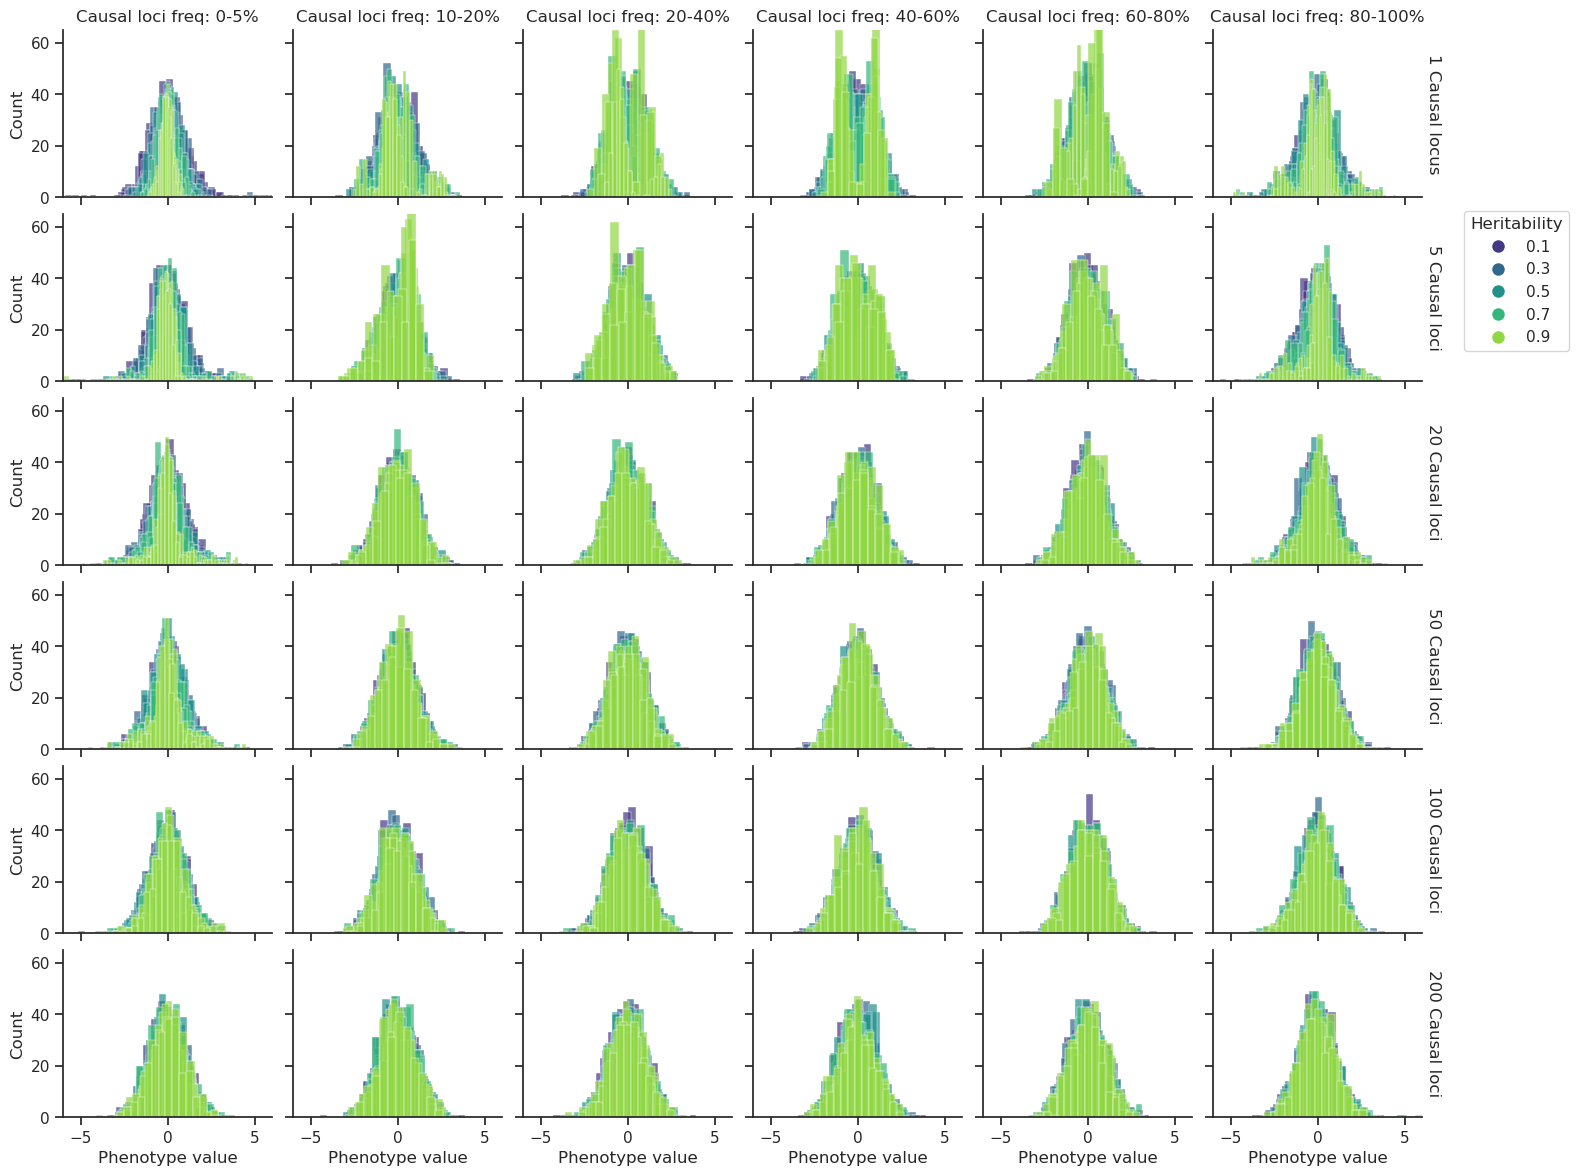
\includegraphics[width=1.1\textwidth]{figures/phenotypes_initial.png}
    \caption{Caption of the figure.}
    \label{fig:phenotypes_initial}
\end{figure}

\begin{figure}[h]
    \centering
    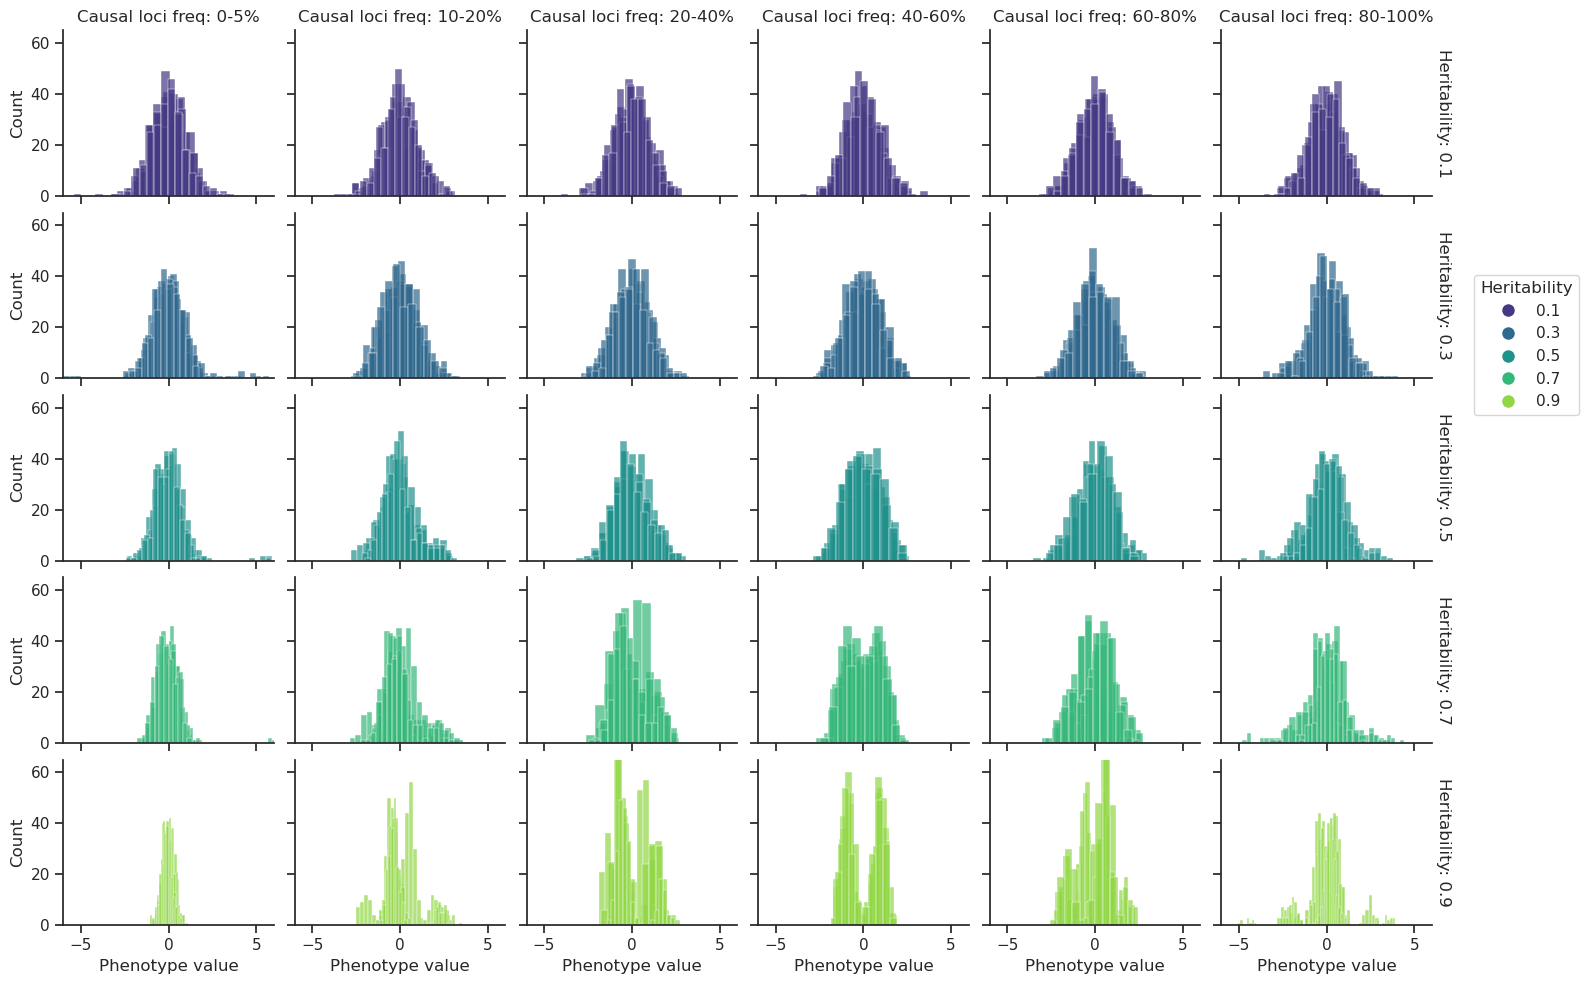
\includegraphics[width=1\textwidth]{figures/phenotypes_initial_onlymonogenic (1).png}
    \caption{Caption of the figure.}
    \label{fig:phenotypes_initial_mono}
\end{figure}

\section{Discussion}

the trait. In the opposite case of mostly large effects, rapid fixations (leading to selective sweeps) may produce fast phenotypic responses. In the examples of fast adaptation mentioned in the Introduction, both of these extremes and combinations thereof have occurred.(Jain and Stephan 2017)
More generally, our analysis also provides some new insights into the question whether selective fixations (and thus sweeps) occur at QTL. While Chevin and Hospital (2008) predicted that the probability of selective sweeps is extremely low at QTL (based on a model with one major locus and infinitely many minor loci), others have found sweeps at appreciable frequencies using simulations of various multi-locus models (Pavlidis et al. 2012; Wollstein and Stephan 2014). The prediction of Chevin and Hospital is consistent with our study for mostly small-effect loci and small shifts in the phenotypic optimum. (Jain and Stephan 2017)



\bibliography{paperpile} % Bibliography

\end{document}
